\documentclass[11pt]{article}
\usepackage{ctex}
\usepackage{CJKutf8}
\usepackage[left=1.25in,right=1.25in,top=1in,bottom=1in]{geometry}
\usepackage{graphicx}
\graphicspath{{figures/}}

\usepackage{fontspec}  % for Consolas

\begin{document}
\begin{CJK}{UTF8}{gkai}
	

\section{Ubuntu系统准备}
Ubuntu系统:\texttt{https://ubuntu.com/download\#download}

UEFI:\texttt{https://www.easyuefi.com/}

DiskGenius:\texttt{https://www.diskgenius.com/download.php}

Ultraiso:\texttt{http://www.ultraiso.net}

sudo apt-get install vim

sudo su

\section{Ubuntu屏幕分辨率异常}
\begin{figure}[h]
	\centering
	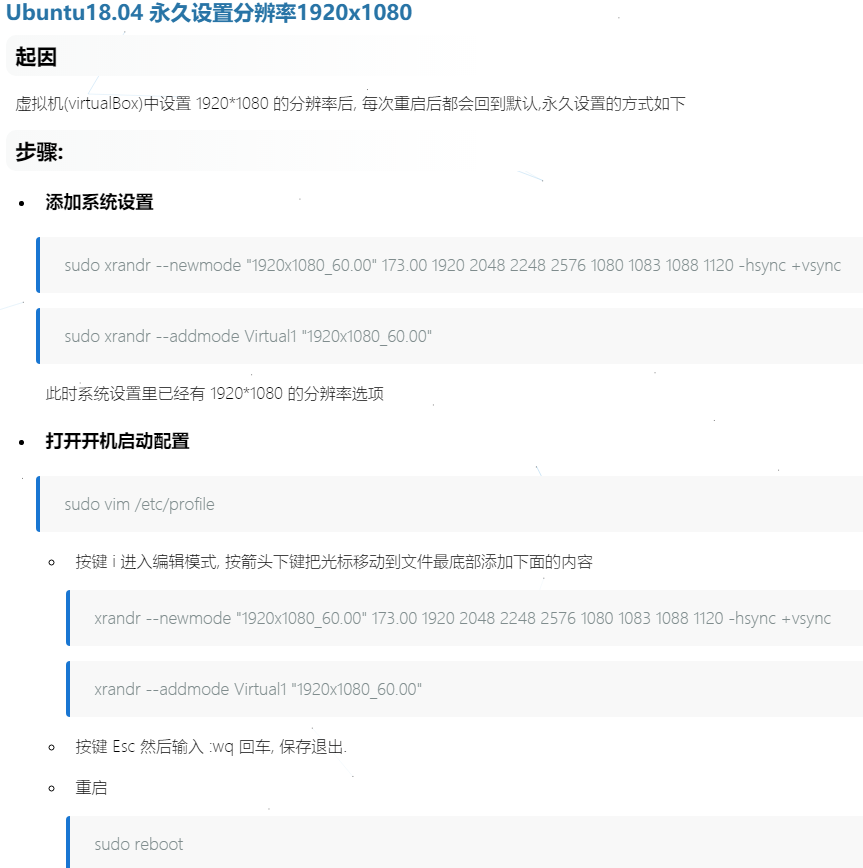
\includegraphics[scale=0.5]{分辨率}
\end{figure}
\begin{figure}[h]
	\centering
	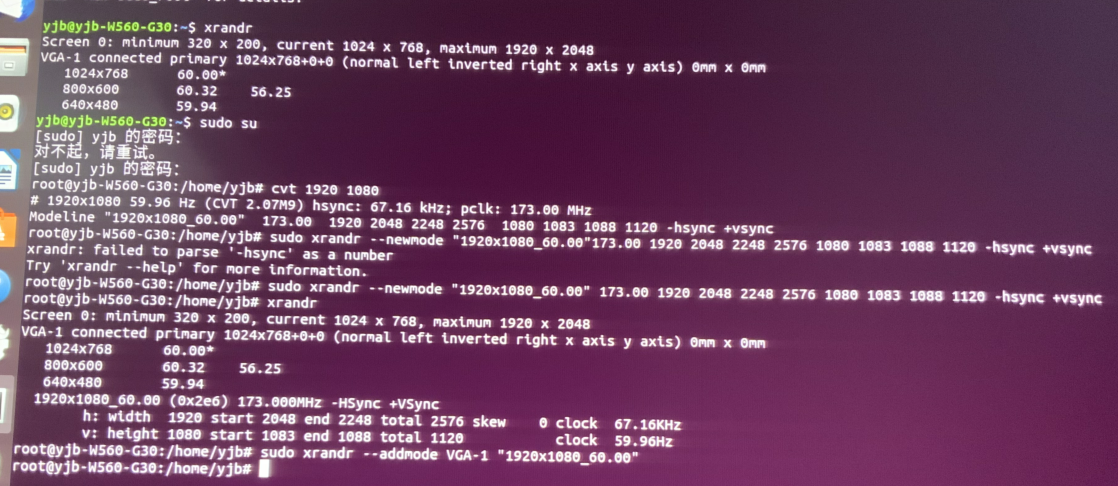
\includegraphics[scale=0.4]{分辨率2}
\end{figure}
\section{配置显卡}
\subsection{禁用nouveau}
1.nouveau开启

lsmod | grep nouveau

2.打开编辑配置文件

sudo gedit /etc/modprobe.d/blacklist.conf

3.在最后一行添加以下命令,禁用第三方驱动

blacklist nouveau

4.使命令生效

sudo update-initramfs -u

5.重启

sudo reboot

6.验证nouveau禁用

lsmod | grep nouveau

\subsection{安装驱动}  
1.查看显卡

ubuntu-drivers devices

2.去NVDIA driver search page(\texttt{https://www.nvidia.com/Download/index.aspx})查看支持显卡的驱动的最新版本的版本号

3.安装相关包

sudo apt update

sudo apt install build-essential

gcc $--$version

4.安装驱动

sudo bash NVIDIA-Linux....run

5.重启电脑

sudo reboot

6.查看安装版本

nvidia-smi

\subsection{安装cuda}

\texttt{https://developer.nvidia.com/cuda-downloads?target\_os=Linux\&target\_arch=x86\_64
	\&Distribution=Ubuntu\&target\_version=18.04\&target\_type=runfile\_local}

sudo sh cuda... --help

nvcc $--$version


sudo vim ~/.bashrc

在该文件中加入以下命令

export CUDA\_HOME=/usr/local/cuda-11.1

export LD\_LIBRARY\_PATH=/usr/local/cuda-11.1/lib64:\$LD\_LIBRARY\_PATH

export PATH=/usr/local/cuda-11.1/bin:\$PATH

source $\sim$/.bashrc

\subsection{安装cudnn}
\texttt{https://developer.nvidia.com/rdp/form/cudnn-download-survey}

选择与cuda 10.1对应的版本(7.6.5),点开后选择 cudnn library for linux,点击下载。(最好选择 cudnn library for linux 这个文件格式安装比较方便)

\#复制cudnn头文件

sudo cp cuda/include/* /usr/local/cuda-11.1/include/

\#复制cudnn的库

sudo cp cuda/lib64/libcudnn* /usr/local/cuda-11.1/lib64/

\#添加可执行权限

sudo chmod +x /usr/local/cuda-11.1/include/cudnn\_version.h(cudnn.h)

sudo chmod +x /usr/local/cuda-11.1/lib64/libcudnn*

\#查看cudnn的版本号

cat /usr/local/cuda/include/cudnn\_version.h | grep CUDNN\_MAJOR -A 2

\section{配置环境}
\subsection{安装Anaconda}
\textbf{Step1}:Update Local Package Manager

sudo apt-get update

sudo apt-get install wget

\textbf{Step2}:Download the latest version of anaconda

https://www.anaconda.com/products/individual-d

or use wget command to download the files

wget https://repo.anaconda.com/archive/Anaconda3-2021.05-Linux-x86\_64.sh

\textbf{Step3}:Verify the download checksum

sha256sum Anaconda3-2021.05-Linux-x86\_64.sh

then your system will display a series of letters and numbers.

\textbf{Step4}:Run anaconda installation script

sudo bash Anaconda3-2021.05-Linux-x86\_64.sh -p /usr/local/ -u 
\begin{figure}[h]
	\centering
	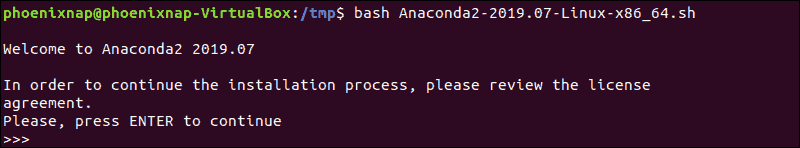
\includegraphics[scale=0.4]{anaconda1}
\end{figure}

\textbf{Step5}:Add the path to the system

sudo gedit $\sim$/.bashrc

\#export PATH= /usr/local/anaconda3/bin:\$PATH

source $\sim$/.bashrc

conda info

\textbf{Step6}:Update anaconda on ubuntu

conda update conda

conda update anconda

\textbf{Step7}:Command about anaconda environments

sudo conda creat $--$name test\_environment python=3.8 

conda info $--$envs

conda activate test\_environment

conda remove $--$name text\_environment $--$all 

解决sudo conda无法创建环境

vim $\sim$/.bashrc

alias sudo="sudo env PATH=\$PATH"

source $\sim$/.bashrc
\section{latex}
\end{CJK}
\end{document}